% !TEX TS-program = XeLaTeX
% use the following command:
% all document files must be coded in UTF-8
\documentclass[spanish]{textolivre}
% build HTML with: make4ht -e build.lua -c textolivre.cfg -x -u article "fn-in,svg,pic-align"

\journalname{Texto Livre}
\thevolume{18}
%\thenumber{1} % old template
\theyear{2025}
\receiveddate{\DTMdisplaydate{2025}{1}{4}{-1}} % YYYY MM DD
\accepteddate{\DTMdisplaydate{2025}{2}{23}{-1}}
\publisheddate{\DTMdisplaydate{2025}{7}{5}{-1}}
\corrauthor{Noemi Fraga-Castrillón}
\articledoi{10.1590/1983-3652.2025.56844}
%\articleid{NNNN} % if the article ID is not the last 5 numbers of its DOI, provide it using \articleid{} commmand 
% list of available sesscions in the journal: articles, dossier, reports, essays, reviews, interviews, editorial
\articlesessionname{dossier}
\runningauthor{Fraga-Castrillón, Couto-Cantero y Trovato} 
%\editorname{Leonardo Araújo} % old template
\sectioneditorname{Hugo Heredia Ponce}
\layouteditorname{Saula Cecília}

\title{Resultados del proyecto InnoTAD:  mejora de las habilidades comunicativas mediante el uso del subtitulado para sordos para aprender lenguas}
\othertitle{Resultados do projeto InnoTAD: melhoria das habilidades comunicativas por meio do uso da legendagem para surdos e ensurdecidos}
% if there is a third language title, add here:
\othertitle{Results of the InnoDAT project:  fostering communicative skills through subtitling for the Deaf and Hard-of-Hearing for learning languages}

\author[1]{Noemi Fraga-Castrillón~\orcid{0000-0003-0178-0208}\thanks{Email: \href{mailto:noemi.fraga.castrillon@udc.es}{noemi.fraga.castrillon@udc.es}}}
\author[1]{Pilar Couto-Cantero~\orcid{0000-0001-7198-6514}\thanks{Email: \href{mailto:pilar.couto@udc.es}{pilar.couto@udc.es}}}
\author[2]{Giuseppe Trovato~\orcid{0000-0002-2225-6010}\thanks{Email: \href{mailto:giuseppe.trovato@unive.it}{giuseppe.trovato@unive.it}}}
\affil[1]{Ciencias de la Educación, Departamento de Didácticas Específicas y Métodos de Investigación y Diagnóstico en Educación, A Coruña, España.}
\affil[2]{Università Ca’ Foscari Venezia, Dipartimento di Studi Linguistici e Culturali Comparati, Treviso, Italia.}

\addbibresource{article.bib}
% use biber instead of bibtex
% $ biber article

% used to create dummy text for the template file
\definecolor{dark-gray}{gray}{0.35} % color used to display dummy texts
\usepackage{lipsum}
\SetLipsumParListSurrounders{\colorlet{oldcolor}{.}\color{dark-gray}}{\color{oldcolor}}

% used here only to provide the XeLaTeX and BibTeX logos
\usepackage{hologo}

% if you use multirows in a table, include the multirow package
\usepackage{multirow}

% provides sidewaysfigure environment
\usepackage{rotating}

% CUSTOM EPIGRAPH - BEGIN 
%%% https://tex.stackexchange.com/questions/193178/specific-epigraph-style
\usepackage{epigraph}
\renewcommand\textflush{flushright}
\makeatletter
\newlength\epitextskip
\pretocmd{\@epitext}{\em}{}{}
\apptocmd{\@epitext}{\em}{}{}
\patchcmd{\epigraph}{\@epitext{#1}\\}{\@epitext{#1}\\[\epitextskip]}{}{}
\makeatother
\setlength\epigraphrule{0pt}
\setlength\epitextskip{0.5ex}
\setlength\epigraphwidth{.7\textwidth}
% CUSTOM EPIGRAPH - END

% to use IPA symbols in unicode add
%\usepackage{fontspec}
%\newfontfamily\ipafont{CMU Serif}
%\newcommand{\ipa}[1]{{\ipafont #1}}
% and in the text you may use the \ipa{...} command passing the symbols in unicode

% LANGUAGE - BEGIN
% ARABIC
% for languages that use special fonts, you must provide the typeface that will be used
% \setotherlanguage{arabic}
% \newfontfamily\arabicfont[Script=Arabic]{Amiri}
% \newfontfamily\arabicfontsf[Script=Arabic]{Amiri}
% \newfontfamily\arabicfonttt[Script=Arabic]{Amiri}
%
% in the article, to add arabic text use: \textlang{arabic}{ ... }
%
% RUSSIAN
% for russian text we also need to define fonts with support for Cyrillic script
% \usepackage{fontspec}
% \setotherlanguage{russian}
% \newfontfamily\cyrillicfont{Times New Roman}
% \newfontfamily\cyrillicfontsf{Times New Roman}[Script=Cyrillic]
% \newfontfamily\cyrillicfonttt{Times New Roman}[Script=Cyrillic]
%
% in the text use \begin{russian} ... \end{russian}
% LANGUAGE - END

% EMOJIS - BEGIN
% to use emoticons in your manuscript
% https://stackoverflow.com/questions/190145/how-to-insert-emoticons-in-latex/57076064
% using font Symbola, which has full support
% the font may be downloaded at:
% https://dn-works.com/ufas/
% add to preamble:
% \newfontfamily\Symbola{Symbola}
% in the text use:
% {\Symbola }
% EMOJIS - END

% LABEL REFERENCE TO DESCRIPTIVE LIST - BEGIN
% reference itens in a descriptive list using their labels instead of numbers
% insert the code below in the preambule:
%\makeatletter
%\let\orgdescriptionlabel\descriptionlabel
%\renewcommand*{\descriptionlabel}[1]{%
%  \let\orglabel\label
%  \let\label\@gobble
%  \phantomsection
%  \edef\@currentlabel{#1\unskip}%
%  \let\label\orglabel
%  \orgdescriptionlabel{#1}%
%}
%\makeatother
%
% in your document, use as illustraded here:
%\begin{description}
%  \item[first\label{itm1}] this is only an example;
%  % ...  add more items
%\end{description}
% LABEL REFERENCE TO DESCRIPTIVE LIST - END


% add line numbers for submission
%\usepackage{lineno}
%\linenumbers

\begin{document}
\maketitle

\begin{polyabstract}
\begin{abstract}
Este artículo se centra en la Traducción Audiovisual Didáctica (TAD) como herramienta útil para la enseñanza del español como segunda lengua extranjera, utilizando la modalidad de Subtitulado para Sordos (SpS) con fines didácticos. El objetivo principal es dar a conocer los resultados obtenidos en el marco del proyecto InnoTAD para demostrar la posibilidad de contribuir a la mejora de las destrezas lingüísticas (comprensión oral y escrita y expresión oral y escrita) a través de la TAD mediante la implementación de seis unidades de aprendizaje (UAs) basadas en el subtitulado para sordos. Para esta investigación se utilizó la metodología del proyecto TRADILEX y el estudio se llevó a cabo en la Università Ca' Foscari (Venecia) con 133 participantes, siendo una parte de la muestra estudiantes del Grado en Mediación Lingüística y Cultural y otra parte, estudiantes del Máster en Traducción e Interpretación. Los datos recogidos en esta investigación sobre destrezas comunicativas son cuantitativos y fueron analizados posteriormente con el programa de análisis estadísticos SPSS. Los resultados obtenidos muestran valores positivos en cuanto a la mejora de cada una de las destrezas comunicativas de la lengua. En la discusión se corroboran esos datos positivos y, en conclusión, este estudio aporta a la comunidad educativa datos empíricos sobre prácticas activas e innovadoras para mejorar la competencia en comunicación lingüística dejando abierta la posibilidad de utilizar otras lenguas y otras modalidades de la TAD para futuras investigaciones.

\keywords{Competencias comunicativas \sep Subtitulado para sordos (SpS) \sep Traducción Audiovisual Didáctica (TAD) \sep Accesibilidad \sep ELE}
\end{abstract}

\begin{portuguese}
\begin{abstract}
Este artigo enfoca a Tradução Audiovisual Didática (TAD) como uma ferramenta útil para o ensino do espanhol como segunda língua estrangeira, utilizando a modalidade de Legendagem para surdos e deficientes auditivos (LSDA) para fins didáticos. O objetivo principal é apresentar os resultados obtidos no âmbito do projeto InnoTAD para demonstrar a possibilidade de contribuir para o aprimoramento das habilidades linguísticas (compreensão oral e escrita e expressão oral e escrita) por meio da TAD mediante a implementação de seis unidades de aprendizagem (UAs) baseadas na legendagem para surdos. Para esta pesquisa, foi utilizada a metodologia do projeto TRADILEX e o estudo foi realizado na Università Ca' Foscari (Veneza) com 133 participantes, sendo uma parte da amostra composta por alunos do curso de Licenciatura em Mediação Linguística e Cultural e a outra parte por alunos do Mestrado em Tradução e Interpretação. Os dados coletados nesta pesquisa sobre habilidades comunicativas são quantitativos e foram posteriormente analisados com o programa de análise estatística SPSS. Os resultados obtidos mostram valores positivos em termos de aprimoramento de cada uma das habilidades comunicativas do idioma. A discussão corrobora esses dados positivos e, em conclusão, este estudo fornece à comunidade educacional dados reais sobre práticas ativas e inovadoras para melhorar a competência de comunicação linguística, deixando em aberto a possibilidade de usar outros idiomas e outras modalidades de TAD para pesquisas futuras.

\keywords{Habilidades de comunicação \sep Legendagem para surdos e deficientes auditivos (LSDA) \sep Tradução Audiovisual Didática (TAD) \sep Acessibilidade \sep ELE}
\end{abstract}
\end{portuguese}
% if there is another abstract, insert it here using the same scheme

\begin{english}
\begin{abstract}
This article focuses on Didactic Audiovisual Translation (DAT) as a useful tool for teaching Spanish as a second foreign language, using the modality of Subtitling for the Deaf and the Hard-of-Hearing (SDH) for didactic purposes. The main objective is to present the results obtained in the framework of the InnoDAT project to demonstrate the possibility of contributing to the improvement of language skills (oral and written comprehension and oral and written expression) through DAT by means of the implementation of six learning units (LUs) based on subtitling for the deaf. For this research, the methodology of the TRADILEX project was used and the study was carried out at the Università Ca' Foscari (Venice) with 133 participants, one part of the sample being students of the Degree in Linguistic and Cultural Mediation and the other part students of the Master's Degree in Translation and Interpreting. The data collected in this research on communicative skills are quantitative and were subsequently analysed with the SPSS statistical analysis programme. The results obtained show positive values in terms of the improvement of each of the communicative language skills. The discussion corroborates these positive data and, in conclusion, this study provides the educational community with real statistics on active and innovative practices to improve linguistic communication competence, leaving open the possibility of using other languages and other modalities of DAT for future research.

\keywords{Communicative skills \sep Subtitling for the Deaf and Hard-of-Hearing (SDH) \sep Didactic Audiovisual Translation (DAT) \sep Accessibility \sep ELE}
\end{abstract}
\end{english}
\end{polyabstract}

\section{Introducción}\label{sec-intro}
Esta investigación pone su centro de interés en la enseñanza y el aprendizaje del español como segunda lengua extranjera en un contexto italiano de educación superior. Para ello, se diseñaron seis Unidades de Aprendizaje (UA) \textit{ad hoc} basadas en la modalidad de traducción audiovisual (TAV) del Subtitulado para Sordos (SpS). Por lo que se refiere a la TAV ya existe mucha literatura y estudios contrastados al respecto. En el pasado se implementaron proyectos sobre TAV con muy buenos resultados: ClipFlair (2011-2014) o PluriTAV (2017-2019). Hoy en día el concepto de Traducción Audiovisual Didáctica (TAD), es decir, el uso de la TAV con fines pedagógicos para aprender lenguas se ha transformado en un enfoque metodológico con mucha potencialidad (TRADILEX, 2020-2023). Por lo tanto, esta investigación contribuye a fomentar la TAD como medio para aprender lenguas extranjeras y cubrir esa brecha de investigación existente. Si bien existía una serie de investigadores que creían que la traducción no era útil para la enseñanza y el aprendizaje de lenguas extranjeras porque la consideran una metodología muy tradicional \cite{lado1964}, conviene indicar que la traducción puede utilizarse de forma muy activa fomentando la interacción en la enseñanza y el aprendizaje de lenguas \cite{fraga-castrillon2024}. 

Además, estas actividades de traducción pueden realizarse en línea e individualmente, de modo que se fomenta el autoaprendizaje y los profesores pasan a desempeñar un papel secundario guiando a los alumnos sólo cuando es necesario. Por lo tanto, los aprendices constituyen el centro del proceso de enseñanza y aprendizaje de lenguas o, dicho de otro modo, se aplica a estos efectos una metodología centrada en el alumno \textit{(Student Centred Curriculum)}. Asimismo, la importancia de este estudio radica en la necesidad de comprobar si los estudios teóricos realmente funcionan cuando se trata de llevarlos a la práctica real en las aulas de aprendizaje, de ahí este estudio empírico. 

Para dar sentido a esta investigación se plantea, por tanto, la siguiente pregunta de investigación (PI): ¿Hasta qué punto el uso de la TAD en la modalidad de SpS favorece la enseñanza y aprendizaje de las destrezas de la lengua objeto de estudio?

Como consecuencia de esta PI formulada se plantean a continuación los siguientes objetivos (O):

\begin{itemize}
    \item (O1) - Comparar los resultados obtenidos en un pretest y postest de destrezas comunicativas tras la realización de UAs basadas en SpS didáctico para el aprendizaje de lenguas extranjeras.
    \item (O2) - Comprobar si existe una mejora significativa en las destrezas comunicativas tras la comparación de los resultados obtenidos en el O1.
\end{itemize}

Para dar respuesta a la PI y cumplir los objetivos planteados, se hizo uso de los datos obtenidos procedentes de un test inicial de destrezas Integradas (TIDI) y un test final de destrezas Integradas (TEFIDI) para determinar si las UAs elaboradas con base en el SpS didáctico pueden ser recomendadas (o no) para mejorar las destrezas comunicativas de la lengua en el contexto mencionado anteriormente. Por otra parte, conviene aclarar que tanto el TIDI como el TEFIDI \cite{fraga-castrillon2021} fueron previamente diseñados bajo los auspicios del proyecto TRADILEX para evaluar todas las destrezas de la lengua de forma integrada: comprensión oral, comprensión escrita, producción oral, producción escrita y mediación de acuerdo con las pautas recomendadas en el Marco Común Europeo de Referencia para las lenguas (MCER) \cite{councilofeurope2018}. 

\section{Marco teórico}\label{sec-2}

\subsection{Traducción Audiovisual y Traducción Audiovisual Didáctica}\label{sec-2.1}
Por lo que respecta a la traducción audiovisual (TAV), cabe mencionar que los primeros estudios sobre traducción surgieron tras la Segunda Guerra Mundial, cuando el aprendizaje de lenguas extranjeras era una obligación debido a la necesidad de comunicación internacional entre los países. A finales de los años 80 surgió un gran debate sobre las diferentes metodologías para el aprendizaje de idiomas \cite{danan2010}. Fue en ese momento cuando la traducción en la enseñanza de lenguas extranjeras reapareció como actividad comunicativa en la vida real ofreciendo la posibilidad de adquirir un aprendizaje significativo, gracias al uso de \textit{realia} o materiales auténticos como, por ejemplo, los vídeos tal y como se puede apreciar en diferentes estudios de \textcite{rivers1978} y \textcite{navarro-pablo2019}. Por otra parte, \textcite{vanderplank1988} fue uno de los pioneros en demostrar que el uso de la traducción a través de un enfoque audiovisual podía ser muy eficaz en la enseñanza y aprendizaje de lenguas extranjeras, demostrando que el uso de la lengua materna en el proceso de aprendizaje de lenguas extranjeras ayuda a su adquisición \cite{fraga-castrillon2021, perez-cabello2024}. Tras estas consideraciones, más investigadores decidieron evaluar el potencial que el uso de estas estrategias podría aportar a la didáctica de las lenguas \cite{araujo2008, danan2004, incalcaterra2014, lertola2012, lertola2013, talavan2013, talavan2019, talavan2020, talavan2024, tinedo-rodriguez2023}. 

En cuanto a la traducción audiovisual didáctica (TAD) conviene indicar que, de acuerdo con \textcite{talavan2013} las diferentes modalidades de TAV: doblaje, subtitulado, audiodescripción, subtitulado para sordos, locución, localización de juegos y voice-over \cite{araujo2008, diazcintas2012, rodriguez-arancon2024, fraga-castrillon2024} pueden ser utilizadas individualmente para la enseñanza y aprendizaje de lenguas maternas y extranjeras. Entre las modalidades anteriormente citadas, existen dos categorías que se incluyen dentro del término que se ha denominado ``accesibilidad audiovisual" que son la audiodescripción (AD) y el subtitulado para sordos y personas con déficit auditivo (SpS) con los que podemos también realizar tareas como recurso pedagógico (TAD) \cite{ogea-espejel2024, ogea-talavan2024}. Todo ello, se debe a que hoy en día podemos hacer uso de una enorme e ilimitada cantidad de contenidos gratuitos en todos los medios de comunicación y esto facilita la implementación de tareas reales y auténticas.

\subsection{El proyecto TRADILEX y el proyecto InnoTAD}\label{sec-2.2}
El proyecto TRADILEX nació como consecuencia de la investigación sobre el uso de la TAV como una potencial herramienta didáctica para la enseñanza y aprendizaje de lenguas. Partiendo de ese objetivo inicial, se llegó a la combinación, el uso de videos y la explotación de recursos tecnológicos de la TAV para darles un uso pedagógico, lo cual derivó en el nacimiento de la TAD explicada en el apartado anterior. Este enfoque didáctico ha sido científicamente probado y, como consecuencia de ello, se ha podido comprobar empíricamente el impacto positivo reflejado en el ámbito de la enseñanza y aprendizaje de lenguas tal y como sugieren \textcite{fernandez-costales2023}, entre otros.

El Proyecto TRADILEX sigue un modelo comunicativo basado en tareas que es compatible con otras metodologías innovadoras como pueden ser: el Aprendizaje Integrado de Contenidos en Lenguas Extranjeras (AICLE), Aprendizaje Basado en proyectos (ABP) o la Clase Invertida. Estas metodologías sitúan al estudiante, que siempre juega un papel activo, en el centro del proceso de aprendizaje en todo momento. Otra característica muy importante es la flexibilidad que estos recursos tienen para generar tareas múltiples y muy variadas adaptadas a los distintos niveles de aprendizaje y, además, también pueden ser llevadas a cabo tanto en la modalidad presencial como en la modalidad en línea, lo cual favorece el aprendizaje guiado por el docente como el aprendizaje autónomo. Por tanto, el principal objetivo del proyecto TRADILEX consiste en integrar el aprendizaje funcional con las destrezas de la lengua incluida la mediación facilitando, a su vez, el desarrollo de la competencia intercultural, la competencia digital y la educación en valores (\url{https://tradit.uned.es/proyecto-tradilex/}). Los resultados positivos obtenidos en el proyecto TRADILEX, tal y como indican \textcite{fernandez-costales2023}, establecen un antes y un después en el desarrollo de futuras investigaciones relacionadas con el ámbito de la TAD.

Posteriormente y en sincronía con este proyecto surge InnoTAD, como un proyecto específico adaptado a un contexto de Educación Superior concreto en el que estudiantes italoparlantes de universidad estudian y aprenden español como segunda lengua extranjera. Asimismo, InnoTAD se centra específicamente en el uso de la modalidad de SpS con el objetivo de obtener nuevos datos y contribuir dentro de la comunidad científica a este campo del aprendizaje de lenguas por medio de la traducción audiovisual didáctica \cite{couto-cantero-trovato2023}. Para poder llevar a cabo este proyecto se creó un cuestionario inicial que fue enviado a los participantes potenciales para conocerlos mejor y poder diseñar las UAs de acuerdo con sus intereses y expectativas. A continuación, se les solicitó completar un TIDI para cada destreza lingüística de modo que las investigadoras pudiesen tener suficientes datos de partida para poder medir las mejoras conseguidas por cada estudiante tras la implementación de las unidades de aprendizaje y así contrastar los datos en el análisis posterior. El siguiente paso consistió en el diseño y ejecución de las seis UAs por parte de los participantes. Estas UAs están basadas en el SpS intralingüístico (se usa la lengua española tanto como \textit{input} como \textit{output} en las tareas) y fueron elaboradas incluyendo diferentes temas de acuerdo con los intereses de los participantes: historia, emociones, turismo, medios de comunicación, entrevistas de trabajo y Navidad.

Las seis UAs fueron diseñadas de acuerdo con la estructura previamente elaborada por los miembros del proyecto TRADILEX \cite{talavan2024}. En primer lugar, la fase de calentamiento \textit{(warm up or pre-task)} en la que se incluyen actividades de comprensión escrita; en la segunda fase \textit{(video watching task)}, se visualiza el video que posteriormente subtitularán; en la tercera fase (AVT task), se incluye el subtitulado didáctico en el que los participantes escriben el texto siguiendo las instrucciones del reglamento UNE153010 y finalmente; la cuarta fase \textit{(post-AVT task)} en la que se practica básicamente la expresión oral. Posteriormente, los participantes completaron el TEFIDI para poder compararlo con los resultados del TIDI. Para finalizar, los participantes cubrieron un cuestionario final donde incluyeron sus percepciones\footnote{Se puede encontrar información en \textcite{couto-cantero-trovato2023} sobre los resultados de las percepciones de los participantes que formaron parte del proyecto mostrando sentimientos positivos en general, tanto sobre su mejora en cuanto a las destrezas comunicativas como su mejora en el conocimiento de la cultura y tradiciones españolas.} sobre la mejora en su aprendizaje de la lengua española y otros comentarios libres sobre su impresión acerca de la propuesta del proyecto InnoTAD. 

\subsection{Subtitulado para sordos (SpS)}\label{sec-2.3}
El subtitulado para sordos (SpS) también conocido como \textit{closed captions} ha evolucionado a lo largo de los años para dotar de accesibilidad e inclusión a ciudadanos con discapacidad auditiva. En sus inicios el SpS constituía un medio para ofrecer únicamente la representación textual de un diálogo, pero con el tiempo ha ido evolucionando para incluir más información tal como: efectos sonoros, información sobre el contexto, datos sobre la entonación o descripciones musicales. Algunos países ya han establecido reglamentos y estándares para el SpS con el objetivo de garantizar la accesibilidad a programas de televisión, películas, plataformas de entretenimiento y todo tipo de contenidos en línea a una audiencia más amplia \cite{aenor2012}.

En España, la normativa estándar UNE153010 \cite[p. 4]{aenor2012} es el documento que: ``establece un mínimo de requerimientos de calidad y un grado razonable de homogeneidad en el subtitulado para sordos". Por lo tanto, el objetivo consiste en eliminar barreras tal y como indica la agenda aprobada por las Naciones Unidas \citeyear{un2015} que adoptó los Objetivos de Desarrollo Sostenible 2030. Específicamente se pretende potenciar la accesibilidad como una herramienta poderosa para garantizar a las personas con discapacidad auditiva que se cumpla el artículo 27 de la Declaración de los Derechos Humanos \cite{un1948}. Este artículo establece que todo el mundo tiene derecho a acceder, participar y disfrutar de las artes y de cualquier actividad dentro de la vida cultural de la comunidad en la que vive.

Para poder hablar del SpS como una modalidad de la DAT es necesario profundizar el subtitulado intralingüístico como una herramienta de aprendizaje \cite{vanderplank1988}. Los subtitulados intralingüísticos a los que podemos acceder en los materiales audiovisuales disponibles contienen, además de la información suprasegmental y la información no verbal diseñada para la comunidad de discapacitados auditivos, interpretaciones escritas de los diálogos hablados que son también útiles para los aprendices de lenguas extranjeras o segundas lenguas. De acuerdo con \textcite{gambier2015}, la redundancia de información a la que el oyente accede a través de múltiples inputs semióticos es especialmente útil para los aprendices con problemas de comprensión auditiva o con problemas de concentración puesto que se combinan tres tipos de información a la vez: la oral, la visual y la escrita. Asimismo, sirve también de gran ayuda para los aprendices con un estilo de aprendizaje más visual que auditivo \cite{tarquini2016}. Por otra parte, varios estudios en los que se utiliza el SpS como un producto de traducción audiovisual didáctico de forma activa, es decir, el aprendiz es el que produce activamente los subtítulos de un texto, confirman todo lo mencionado anteriormente \cite{talavan2019, talavan2020, talavan2022, couto-cantero-trovato2023}.

Dentro de ese mismo marco, \textcite{zarate2021} indica que los principales retos de los aprendices que utilizan el SpS didáctico consisten en que deben esforzarse por identificar a los distintos hablantes (mediante colores, etiquetas o directrices), la música (incluida la letra), los efectos sonoros (incluidos los sonidos vocales no-verbales relacionados con acciones o emociones) y otros rasgos paralingüísticos como: la pronunciación, la entonación, el acento, el sarcasmo, los susurros y las situaciones. Por último, este artículo se basa en el proyecto InnoTAD, en el que los participantes completaron una serie de unidades de aprendizaje basadas en el SpS intralingüístico (audio en español y subtitulado en español) así como los TIDI y TEFIDI descritos anteriormente.

\section{Metodología}\label{sec-3}
InnoTAD es un proyecto de investigación experimental en el que se procura comprobar la mejora de aprendizaje de la lengua española como segunda lengua extranjera a través de una serie de unidades de aprendizaje. El proyecto se llevó a cabo en el año académico 2022-2023 siguiendo la metodología de aprendizaje en línea de TRADILEX. Para dar respuesta a nuestra pregunta de investigación: ¿Hasta qué punto el uso de la TAD en la modalidad de SpS favorece la enseñanza y aprendizaje de las destrezas de la lengua objeto de estudio?, se realizó un estudio comparativo cuantitativo. Los datos se obtuvieron, por un lado, de los resultados previos a la ejecución de las unidades de aprendizaje conseguidos a través de un TIDI y, por otro lado, de los resultados obtenidos del TEFIDI.

\subsection{Participantes}\label{sec-3.1}
Esta investigación consta de una muestra intencional de un total de 133 estudiantes universitarios italoparlantes de la Università Ca’ Foscari (en Venecia, Italia). El 40,6 \% de los participantes estudian un grado en Mediación Lingüística y Cultural y, el 59,4 \%, estudios de máster de Traducción Especializada. La mayoría del alumnado (93,7 \%) tiene entre 18 y 25 años, mientras que los restantes no superan los 30. 

En lo que atañe al conocimiento previo de lenguas, el 95 \% tienen como lengua materna el italiano junto con el dialecto correspondiente a la región en la que viven. Solamente el 5 \% son bilingües nativos en italiano y otra lengua, como el francés, albanés, bosnio, árabe, polaco o rumano. Por otro lado, el nivel de conocimiento de la lengua española previo a la puesta en marcha del proyecto InnoTAD, siguiendo el Marco Común Europeo de Referencia para las Lenguas (MCER), ha sido mayoritariamente el nivel B2 (64 \%), seguido del B1 (28,5 \%) y un 7,5 \% que no tiene ningún nivel certificado. Además, se ha confirmado que muy pocos participantes habían realizado con anterioridad actividades de TAD en clase o fuera de ella (12 \%), en comparación con el 88 \% que reconocen saber en qué consiste la TAD, pero admiten que nunca han tenido la oportunidad de practicar ninguna actividad del estilo.

\subsection{Materiales e instrumentos de recogida de datos}
Los materiales utilizados en el proyecto InnoTAD han sido adaptados del proyecto TRADILEX \cite{couto-cantero2021}, enfocándolos a nuestro objeto de estudio: el aprendizaje del español como lengua extranjera. Para responder la pregunta de investigación, los materiales utilizados han sido: a) Un TIDI (comprensión escrita, expresión escrita, comprensión oral y expresión oral), b) seis UAs basadas en el SpS, c) un TEFIDI (comprensión escrita, expresión escrita, comprensión oral y expresión oral). En este artículo no se hace especial hincapié en las cualificaciones de cada UA, ya que nuestro objetivo es realizar una comparación entre el nivel de lengua española antes de realizar las actividades que llevaron a cabo y el nivel posterior a la elaboración de dichas actividades.

Tanto los TIDI como los TEFIDI duran aproximadamente 20 minutos cada uno. En los test de comprensión escrita, los participantes deben leer un texto corto sobre un contenido específico y responder a las preguntas para comprobar el entendimiento del texto. Por otro lado, en los test de expresión escrita, se ofrece al alumnado un texto o un vídeo corto sobre un argumento en concreto y ellos redactan un párrafo con su opinión sobre el tema. Cabe destacar que el diseño de los test iniciales tiene que ser lo más parecido posible a los test finales para que la única diferencia que se aprecie sea la mejora (o no) de la lengua, sin que exista ningún otro factor que pueda perjudicar los resultados, como por ejemplo el tipo de actividad o el contenido.

\subsection{Procedimiento}\label{sec-3.3}
El instrumento de recogida de datos se mostró \textit{in situ} por dos miembros del equipo de investigación durante la primera semana del curso académico 2022-2023 para proporcionar las instrucciones básicas necesarias sobre cómo acceder a los contenidos y cómo completar las tareas, así como para resolver las dudas o problemas planteados por los participantes. Por tanto, los participantes completaron el TIDI y la primera UA de forma presencial en el aula con la ayuda de los investigadores y finalizaron las otras cinco UAs y el TEFIDI en línea durante las semanas siguientes antes de terminar el primer semestre. Se habilitaron diferentes vías (chats, foro, correo electrónico, etc.) para que los estudiantes resolvieran cualquier duda o pregunta sobre el procedimiento durante este proceso. Asimismo, los investigadores ofrecieron una retroalimentación individualizada por correo electrónico a medida que los estudiantes iban completando cada unidad de aprendizaje.

Para llevar a cabo con éxito el proyecto InnoTAD, los estudiantes completaron primero las pruebas TIDI de las cuatro destrezas. Cada parte del TIDI tuvo una duración aproximada de 20 minutos y correspondía a una habilidad comunicativa específica, de modo que, en 80 minutos, los participantes realizaron las pruebas correspondientes a: comprensión oral, expresión oral, comprensión escrita y expresión escrita. Posteriormente, se efectuaron las seis lecciones del plan didáctico SpS. Como ya se ha citado anteriormente cada UA estaba compuesta por cuatro secciones: (1) actividades de calentamiento, (2) actividades de previsualización, (3) actividad principal basado en el SpS didáctico y (4) actividades posteriores al proceso de TAD.

En la primera sección de calentamiento, se proporcionó a los estudiantes un texto y preguntas formuladas concretamente para el nivel B2 según el MCER. A continuación, realizaron una previsualización del video, en el cual añadieron subtítulos y respondieron algunas preguntas breves con el objetivo de familiarizarse con el vocabulario, el tono de voz o el acento, entre otros aspectos, para facilitar la actividad principal. Posteriormente, en la actividad principal, los estudiantes debían subtitular un video en el programa Aegisub, y para ello se les brindó una serie de pautas junto con enlaces a archivos de video y subtítulos (.ass o .srt) para su descarga y apertura en Aegisub de manera sencilla. Finalmente, en las actividades posteriores al proceso de traducción audiovisual didáctico, se les presentó un video relacionado con el tema principal de la unidad de aprendizaje y realizaron una grabación de audio con el programa Vocaroo para expresar sus opiniones o debatir sobre el tema.

En lo que concierne a las unidades de aprendizaje, es importante señalar que estas fueron diseñadas siguiendo la taxonomía de Bloom \cite{anderson2001} para incrementar progresivamente el grado de dificultad, de modo que la primera UA fue percibida como más sencilla en comparación con la sexta. Además, cada unidad abordó un tema principal sobre el que se organizaron todas las actividades: en la primera, historia/cultura de España; en la segunda, las emociones; en la tercera, el turismo y la cultura (Camino de Santiago); en la cuarta, los medios de comunicación; en la quinta, información sobre cómo hacer una entrevista de trabajo; y en la última, cultura y fiestas españolas (la Navidad). La selección de estos contenidos se basó, por un lado, en los intereses manifestados por los estudiantes a través de un cuestionario previo y, por otro, en el deseo de incluir tanto temas culturales como ciertos eventos históricos, el Camino de Santiago o las festividades navideñas en España.

Para concluir el proyecto, los estudiantes completaron el TEFIDI. Del mismo modo que el test inicial, este tuvo una duración de aproximadamente 80 minutos, con 20 minutos destinados a cada habilidad evaluada. En cuanto a la organización temporal del proyecto completo, se dividió en dos fases, ya que una parte de los estudiantes cursó la asignatura en la que se implementó el proyecto InnoTAD en el primer semestre, mientras que la otra parte la cursó en el segundo semestre. Por lo tanto, la primera fase se extendió de octubre de 2022 a enero de 2023, mientras que la segunda fase tuvo lugar de febrero a junio de 2023.

\subsection{Análisis de datos}\label{sec-3.4}
Para analizar los datos se ha utilizado el Statistical Package for Social Sciences (SPSS. v.28 IBM Corp., Armonk, NY, USA). En primer lugar, se llevó a cabo un análisis estadístico descriptivo básico para determinar las condiciones de normalidad. Después, se representan los datos de los resultados en histogramas para reconocer la distribución que presentan y, finalmente, se aplica el test no paramétrico de Wilcoxon para el análisis inferencial.

\subsection{Validación, pilotaje, código de conducta y buenas prácticas}\label{3.5}
Por último, cabe mencionar que todos los instrumentos diseñados para este estudio fueron validados por dos expertas en el área objeto de estudio a nivel internacional y probados por otros participantes en una fase piloto previa \cite{couto-cantero2021}. Además, esta investigación y su procedimiento se realizaron de acuerdo con la Declaración de Helsinki y fueron aprobados por el Comité de Ética de las dos universidades involucradas en el proyecto. Asimismo, se cuenta con la aprobación del Comité de Ética de la UNED (5 de julio de 2021) donde se indica que el proyecto titulado: ``La traducción audiovisual como recurso didáctico en el aprendizaje de Lenguas Extranjeras. TRADILEX" cumple todos los requisitos de idoneidad requeridos para proyectos que implican investigación con humanos.

\section{Resultados}\label{resultados}
En esta sección, los resultados se han dividido en subapartados para exponer claramente lo que se presenta de acuerdo con los objetivos anteriormente mencionados.

\subsection{Resultados del O1: comparar los resultados obtenidos en un pre y post test de destrezas comunicativas tras la realización de unidades de aprendizaje basadas en SpS didáctico para el aprendizaje de lenguas extranjeras}\label{sec-4.1}
Para empezar, es necesario exponer los estadísticos descriptivos básicos como la Media, la desviación típica o los límites inferiores y superiores del 95 \% de intervalo de confianza para la media (ver Tabla \ref{tab-1}). Estos datos muestran que la media en todas las pruebas es alta, en torno al 9, excepto en el TIDI EE (8,67). En cuanto a la desviación típica, está en un rango de entre medio punto y un punto ya que la muestra es prácticamente homogénea en cuanto al nivel que poseen de la lengua española.

%---- CÓDIGO DA TABELA 1 ----%
\begin{table}[ht]
\centering
\begin{threeparttable}
\caption{Estadísticos descriptivos básicos.}\label{tab-1}
\begin{tabular}{lcccc}
\toprule
 & Media & Lím. inferior & Lím. superior & Desv. Est. \\
\midrule
TIDI CO     & 9,39 & 9,17 & 9,62 & 1,05 \\
TEFIDI CO   & 9,60 & 9,40 & 9,79 & 0,91 \\
TIDI EO     & 9,00 & 8,81 & 9,19 & 0,92 \\
TEFIDI EO   & 9,16 & 8,98 & 9,34 & 0,86 \\
TIDI CE     & 9,22 & 9,08 & 9,35 & 0,65 \\
TEFIDI CE   & 9,33 & 9,17 & 9,50 & 0,78 \\
TIDI EE     & 8,67 & 8,43 & 8,92 & 1,16 \\
TEFIDI EE   & 9,18 & 9,06 & 9,22 & 0,56 \\
\bottomrule
\end{tabular}
\source{Elaboración propia.}
\notes{Límites inferior y superior con 95 \% de intervalo de confianza para la media. \\
CO = Comprensión oral; EO = Expresión oral; CE = Comprensión escrita; EE = Expresión escrita.}
\end{threeparttable}
\end{table}

Una vez conocidos los datos estadísticos descriptivos, se realiza un análisis de normalidad que sirve para conocer en qué rango se concentran los resultados.

Unos resultados que cumplen las condiciones de normalidad se pueden visualizar fácilmente porque se representan en histogramas con una forma característica de campana (campana de Gauss). En este caso, se realizó el análisis de normalidad de Kolmogorov-Smirnov y Shapiro-Wilk en cada uno de los test de competencias comunicativas y, como se muestra en la Tabla \ref{tab-2}, el valor $p$ es en todos los casos <0,001. Esto indica que los datos no siguen las condiciones de normalidad.

%---- CÓDIGO DA TABELA 2 ----%
\begin{table}[ht]
\centering
\begin{threeparttable}
\caption{Test de normalidad.}\label{tab-2}
\begin{tabular}{lcccccc}
\toprule
 & \multicolumn{3}{c}{Kolmogorov-Smirnov} & \multicolumn{3}{c}{Shapiro-Wilk} \\
\cmidrule(lr){2-4} \cmidrule(lr){5-7}
 & Estadístico & gl & Sig. & Estadístico & gl & Sig. \\
\midrule
TIDI CO     & 0,283 & 89 & <0,001 & 0,593 & 89 & <0,001 \\
TIDI EO     & 0,169 & 89 & <0,001 & 0,880 & 89 & <0,001 \\
TIDI CE     & 0,203 & 89 & <0,001 & 0,851 & 89 & <0,001 \\
TIDI EE     & 0,184 & 89 & <0,001 & 0,889 & 89 & <0,001 \\
TEFIDI CO   & 0,435 & 89 & <0,001 & 0,511 & 89 & <0,001 \\
TEFIDI EO   & 0,182 & 89 & <0,001 & 0,852 & 89 & <0,001 \\
TEFIDI CE   & 0,330 & 89 & <0,001 & 0,743 & 89 & <0,001 \\
TEFIDI EE   & 0,115 & 89 & <0,001 & 0,935 & 89 & <0,001 \\
\bottomrule
\end{tabular}
\source{Elaboración propia.}
\end{threeparttable}
\end{table}

A continuación (ver Figura \ref{fig-1}), se visualiza de manera muy clara que el tipo de distribución de nuestros resultados muestra una curva ascendente hacia la derecha, lo que corresponde con el valor mayor (el 10). A este tipo de distribución donde los datos se concentran en la puntuación más alta se le conoce como distribución con asimetría negativa. Este histograma sirve como ejemplo ilustrativo de cómo se verían todos los resultados ilustrados de los test iniciales y finales.

\begin{figure}[h!]
\centering
\begin{minipage}{0.90\linewidth}
    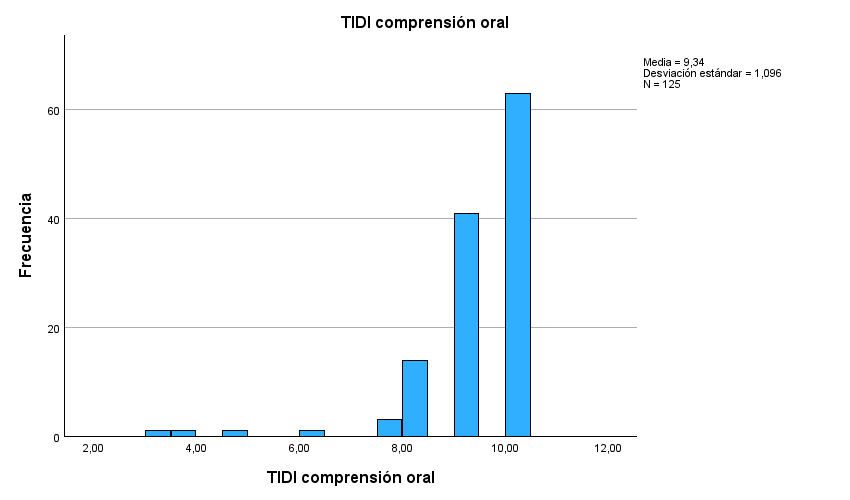
\includegraphics[width=\linewidth]{image1.png}
    \caption{Histograma: distribución de los resultados del TIDI comprensión oral.}
    \label{fig-1}
    \source{Elaboración propia.}
    \notes{Media = 9,34; Desviación estándar = 1,096; N = 125.}
\end{minipage}
\end{figure}

\subsection{Resultados del O2: comprobar si existe una mejora significativa en las destrezas comunicativas tras la comparación de los resultados obtenidos en el O1}\label{sec-4.2}
Para ser capaces de deducir si existe o no una mejora significativa en las destrezas comunicativas, se lleva a cabo el análisis inferencial. Para ello, es esencial tener en cuenta tanto el tamaño de la muestra como el análisis de normalidad. Dado que los resultados obtenidos de esta investigación no cumplen las condiciones de normalidad, como se ha demostrado anteriormente, se debe optar por pruebas no paramétricas. En este caso, el análisis del impacto de la intervención se realizó mediante la comparación de medias. Con ese propósito, se realizó la prueba de Wilcoxon para muestras emparejadas, como se muestra en la Tabla \ref{tab-3}.

%---- CÓDIGO DA TABELA 3 ----%
\begin{table}[ht]
\centering
\begin{threeparttable}
\caption{Test Estadístico Wilcoxon.}\label{tab-3}
\begin{tabularx}{\textwidth}{l *{4}{>{\centering\arraybackslash}X}}
\toprule
 & TIDI-TEFIDI CO & TIDI-TEFIDI EO & TIDI-TEFIDI CE & TIDI-TEFIDI EE \\
\midrule
Z                     & -1,185 & -4,670 & -0,397 & -3,573 \\
Sig. Asin. (bilateral) & 0,236  & <0,001 & 0,692  & <0,001 \\
\bottomrule
\end{tabularx}
\source{Elaboración propia.}
\end{threeparttable}
\end{table}

Una vez aplicada la prueba no paramétrica de Wilcoxon, se obtiene un valor $p$ < 0,001 en las parejas TIDI-TEFIDI EO y TIDI-TEFIDI EE, lo que significa que hay pruebas suficientes para expresar que las unidades de aprendizaje son eficaces para mejorar las habilidades de expresión oral y expresión escrita a un nivel de significación del 1 \%. En otras palabras, hay un 99 \% de posibilidades de asegurar que las UAs aplicadas fueron eficaces para la mejora de dichas destrezas. Por el contrario, en las parejas TIDI-TEFIDI CO y TIDI-TEFIDI CE el valor $p$ es de 0,236 y 0,692 respectivamente. En este caso, no se puede afirmar que haya una mejora significativa a un nivel de significación del 1 \%.

\section{Discusión y conclusiones}
Para comenzar este apartado de discusión y conclusiones, conviene mencionar que la motivación fue lo suficientemente elevada como para que el 70,7 \% de los estudiantes completaran todas las actividades incluidas en el proyecto y todo ello a pesar de tratarse de un proyecto en línea en su mayor parte. Por lo tanto, se puede verificar que el grado de compromiso en la realización de este proyecto fue muy alto, si se tiene en cuenta que, en general, en las universidades de educación a distancia que utilizan la modalidad en línea para impartir clases, la tasa de seguimiento suele ser inferior al 40 \%. Asimismo, en este contexto de aprendizaje a distancia y, de acuerdo con García-Aretio, podemos estar de acuerdo en que la ``tasa de éxito" es aquella en la que los estudiantes completan todas las tareas disponibles en los cursos, o proyectos incluyendo las tareas de evaluación final \citeyear{garcia-aretio2017}. Además, como afirmó \textcite{tarquini2016} se ha comprobado que el Proyecto InnoTAD también ha sido de gran ayuda para los alumnos que tenían un estilo de aprendizaje más visual que auditivo. Del mismo modo, tener acceso a múltiples informaciones semióticas \cite{gambier2015} ha demostrado ser muy útil para los participantes, ya que fueron capaces de combinar las entradas de información orales, visuales y escritas para completar las tareas TAD.

Como ya se ha mencionado en el marco teórico, \textcite{vanderplank1988} fue uno de los pioneros en demostrar que el uso de la traducción a través de un enfoque audiovisual podía ser muy eficaz en la enseñanza y el aprendizaje de lenguas extranjeras. No solo el proyecto InnoTAD ha demostrado estar en la línea con esta afirmación que cobra peso desde hace tantos años, sino que varios estudios actuales como los de \textcite{talavan2019}, \textcite{talavan2022} o \textcite{couto-cantero-trovato2023} van en la misma dirección. El aprendizaje significativo también se consiguió en este proyecto gracias al uso de realia o materiales auténticos. En consecuencia, los vídeos incluidos en todas las unidades de aprendizaje desempeñaron un papel muy importante para cumplir este objetivo, como ya se ha señalado en estudios anteriores \cite{navarro-pablo2019} y también en la actualidad \cite{couto-cantero2023}. Además, el hecho de incluir simulaciones basadas en situaciones reales, así como entrevistas orales y presentaciones \cite{garcia-carbonell2001, angellini2012} fue también una ganancia para acometer este proyecto con éxito.

En el proyecto InnoTAD, en el que se ha utilizado el SpS como herramienta activa de TAD, los participantes tuvieron que esforzarse para identificar los personajes, la música, los efectos de sonido y otros rasgos paralingüísticos como la pronunciación, la entonación, el acento, el sarcasmo, los susurros y las situaciones inesperadas. Este fue uno de los principales retos que tuvieron que resolver los participantes y es lo mismo que afirmaron otros investigadores como \textcite{zarate2021} a la hora de hablar del tratamiento de las actividades y tareas de SpS. 

A primera vista, si se atiende a la diferencia de las notas entre el test inicial y el final, se podría considerar que no hay una mejora significativa en las habilidades de ``comprensión", tanto oral como escrita, porque el valor del TEFIDI no aumenta mucho en relación con el TIDI. Sin embargo, para realizar un buen análisis es conveniente profundizar en los datos para discutir los resultados. De esta forma, se puede constatar que ha habido una mejora importante porque la puntuación media inicial del TIDI ya era sustancialmente alta, por lo que estos autores corroboran que la mejora sólo podría aumentar 0,61 puntos como máximo en el caso de la comprensión oral y 0,78 puntos en la comprensión escrita. Sabiendo esto, el aumento medio de 0,21 puntos en el TEFIDI correspondería a una mejora del 34,43 \% (en la comprensión oral) y el aumento medio de 0,78 puntos correspondería a una mejora del 14,10 \% (en la comprensión escrita), lo cual es un porcentaje interesante para tener en cuenta. Además, en lo que concierne a la mejora de las habilidades de expresión, tanto oral como escrita, los resultados muestran una mejora significativa. Por lo tanto, a la luz de los resultados, se confirma rotundamente que con las UAs del proyecto InnoTAD se mejoran significativamente las habilidades de expresión oral y de expresión escrita dentro del contexto universitario con estudiantes italoparlantes.

Por otro lado, es importante resaltar la importancia de un buen diseño de las UAs como punto clave para mejorar las destrezas lingüísticas en un proyecto como InnoTAD que se basa en la modalidad de SpS. La actividad principal del proyecto consistía en la realización de una tarea de SpS y, como de todos es sabido, en la realización del SpS no se practica la expresión oral, pero con una buena elección de las actividades anteriores y posteriores a la misma, se pudo planificar el desarrollo también de la expresión oral o de la lectura (habilidades que no estaban incluidas en la tarea principal). Por tanto, se puede afirmar, sin miedo a equivocarse, que los datos aportados en este estudio al implementar las UAs del proyecto InnoTAD basadas en la modalidad de SpS suponen una clara representación que confirma que es posible que el alumnado consiga una mejora en el aprendizaje de las destrezas de la lengua. Estos excelentes resultados se hicieron efectivos gracias a una buena planificación y diseño de las actividades, lo que fue posible al tener en cuenta la retroalimentación previa proporcionada por los participantes \cite{bygate2009teaching}. Incluir tareas específicas señaladas por los participantes, como entrevistas de trabajo, también fue un acierto claramente demostrado y permitir que grabaran solos la tarea oral – sin que un profesor les interrumpiera con correcciones – también fue una decisión muy positiva \cite{romaine2005}.

Aunque los resultados presentados sobre la implementación del Proyecto InnoTAD para la mejora de las destrezas de la lengua han sido positivos, se recomienda no sólo utilizar una modalidad de TAD, sino combinar varias modalidades como el subtitulado, el doblaje, la locución o la audiodescripción \cite{talavan2024}. En ese caso, se considera que, por falta de tiempo, sería probable que hubiese que reducir el número de UAs para cada modalidad. En cuestiones similares, \textcite{fernandez-costales2023} observaron que la mejora tanto en las destrezas orales como en las otras destrezas de la lengua era significativa y, sobre todo, los resultados en el TEFIDI se homogeneizaban en los valores más altos.

Con respecto a las limitaciones de esta investigación, cabe mencionar que una de las debilidades del estudio consiste en que todos los participantes de la muestra tenían el mismo nivel de español y consideramos que sería muy interesante tener más diversidad en cuanto a niveles lingüísticos y poder diseñar las UAs y las pruebas iniciales y finales de acuerdo con cada nivel. También sería muy pertinente comparar en cuáles hay mayor o menor mejora. Por otra parte, se sugiere también la posibilidad de incluir participantes de diferentes lenguas maternas para hacer una comparación entre los aprendices de español como lengua extranjera que proceden de una lengua materna romance, o los que proceden de una anglosajona y comprobar las diferencias entre unos y otros. No obstante, estas limitaciones pueden transformarse en oportunidades y también como un ejemplo de lo que puede hacerse en relación con el tema objeto de estudio de este artículo. La transferibilidad de esta investigación está disponible siempre y cuando los investigadores sean capaces de adaptar esta propuesta a cualquier muestra de participantes y a cualquier lengua meta.

En futuras investigaciones se llevará a cabo el análisis cuantitativo de los resultados obtenidos en el proyecto InnoTAD aplicando otras modalidades de la TAD en las unidades de aprendizaje o en otras lenguas objeto de estudio. De esta forma, se cierra nuestra aportación al campo de la TAD sobre los datos obtenidos con el proyecto InnoTAD en este ámbito del aprendizaje del español como segunda lengua extranjera en Italia mediante actividades de SpS que permanecía vacío hasta la fecha.

\section*{Financiación}\label{sec-organizacao}
El presente estudio ha sido financiado por el proyecto TRADILEX PID 2019 107362 GA I 00 AEI/ 10 13039 501100011033 del Ministerio de Ciencia e Innovación, Gobierno de España. 

Programa de ayudas para estancias predoctorales de investigación INDITEX-UDC 2023.

\printbibliography\label{sec-bib}
% if the text is not in Portuguese, it might be necessary to use the code below instead to print the correct ABNT abbreviations [s.n.], [s.l.]
%\begin{portuguese}
%\printbibliography[title={Bibliography}]
%\end{portuguese}


%full list: conceptualization,datacuration,formalanalysis,funding,investigation,methodology,projadm,resources,software,supervision,validation,visualization,writing,review
\begin{contributors}[sec-contributors]
\authorcontribution{Noemi Fraga Castrillón}[datacuration,formalanalysis,funding,methodology,software,writing]
\authorcontribution{Pilar Couto-Cantero}[conceptualization,funding,supervision,validation,review]
\authorcontribution{Giuseppe Trovato}[investigation,projadm,resources,supervision,visualization]
\end{contributors}




\end{document}